\chapter{Experiment: Partial grouping by amplitude- and
frequency-modulation\label{chap:amfmsep}}

\section{Introduction}
To evaluate whether the grouping of partials with common AM and FM parameters is
plausible, we synthesize a set of parameters and test by corrupting the
parameters with noise and adding spurious sets of parameters that should not
belong to any sources.

\section{Methodology}
We assume parameters have been estimated already so we start from theoretical
values for the amplitude, frequency, frequency modulation and amplitude
modulation.  On each frame of analysis data, i.e., for parameters belonging to
the same time instant, we consider each data-point as a multi-dimensional random
variable. With these random variables, we compute principal components in order
to produce a variable with maximum variance. This variable is classified using a
clustering algorithm and we evalutate the results. A summary follows:
\begin{itemize}
    \item 
        Parameters are synthesized from a theoretical mixture of AM and FM
        sinusoids.  Spurious data are added to these parameters.
    \item
        Principal components analysis is carried out on the parameters happening
        at one time instance.
    \item
        A histogram is made of the first principal components. Values sharing a
        bin with too few other values are discarded to remove spurious data
        points.
    \item
        Initial means and standard deviations for the Gaussian mixture models
        are made by dividing the histogram into equal parts by area and choosing
        the centres of these parts.
    \item
        The EM algorithm for Gaussian mixture models is carried out to classify
        the sources.
\end{itemize}
\section{Evaluation}
The algorithm is run on a typical source separation problem to evaluate its
plausibility. Two sources are synthesized, each exhibiting both frequency- and
amplitude-modulation. The amplitude and frequency of the frequency-modulation
are chosen to be realistic with respect to acoustic sounds --- $\pm12.5$ cents
surrounding the fundamental at around $6$ Hz (see
Table~\ref{tab:synthparamamfmsep}), similar to the measurements obtained in
\cite{mellody2000time} for violin vibrato. Because musical sounds exhibit a wide
variety of amplitude envelopes, one was chosen that seemed realistic, but that
was not based on any particular instrument or recording. For this
process all that is important to carry out source separation is the relative
amplitude modulation of the two sources. 

To have control over the frequency- and amplitude-modulation separately, we
compute the parameters of a function describing the amplitude envelope, and one
describing oscillatory part. The parameters are combined when carrying out the
classification.

% Plots produced in this section with signal_modeling/test/plot_all_am_fm_sep.sh
\begin{figure}[!t]
    \centering
    \includegraphics[width=\figwidthscale\textwidth]{plots/{hsrp_test_7_multi_orig_data}.eps}
    \CaptionWithTitle{%
        \input{plots/hsrp_test_7_multi_orig_data_plot_title.txt}%
    }{Line-segments describing the frequency and frequency modulation
    of both sources with no added spurious parameters.\label{plot:hsrp_test_7_multi_orig_data}}
\end{figure}

\begin{figure}[!t]
    \centering
    \includegraphics[width=\figwidthscale\textwidth]{plots/{hsrp_test_7_multi_orig_spur_data}.eps}
    \CaptionWithTitle{%
        \input{plots/hsrp_test_7_multi_orig_spur_data_plot_title.txt}%
        }{Line-segments describing the frequency and frequency modulation
        of the original data and the spurious data.
    \label{plot:hsrp_test_7_multi_orig_spur_data}}
\end{figure}

\begin{figure}[!t]
    \centering
    \includegraphics[width=\figwidthscale\textwidth]{plots/{hsrp_test_7_multi_class_pcs}.eps}
    \CaptionWithTitle{%
        \input{plots/hsrp_test_7_multi_class_pcs_plot_title.txt}%
        }{The PCs for each theoretical analysis time-point. $\mu_{i}^{0}$ and
        $\sigma_{i}^{0}$ are respectively
    the initial mean and standard deviation guesses for the EM algorithm fitting
    the GMM parameters to the $i$th source. These values are also visible on the
    plot. The spurious points rejected using the process described in
    Section~\ref{sec:amfmseppreparecluster} are included for comparison.
    \label{plot:hsrp_test_7_multi_class_pcs}}
\end{figure}

\begin{figure}[!t]
    \centering
    \includegraphics[width=\figwidthscale\textwidth]{plots/{hsrp_test_7_multi_source_1_est}.eps}
    \CaptionWithTitle{%
        \input{plots/hsrp_test_7_multi_source_1_est_plot_title.txt}%
        }{Line-segments classified as belonging to Source 1. The
        classification is done on each frame so classifications in consecutive
        frames may not belong to the same true source. This is because the
        ordering of the clusters in each frame in
        Figure~\ref{plot:hsrp_test_7_multi_class_pcs} is not predictible.
    \label{plot:hsrp_test_7_multi_source_1_est}}
\end{figure}

\begin{figure}[!t]
    \centering
    \includegraphics[width=\figwidthscale\textwidth]{plots/{hsrp_test_7_multi_source_2_est}.eps}
    \CaptionWithTitle{%
        \input{plots/hsrp_test_7_multi_source_2_est_plot_title.txt}%
        }{Line-segments classified as belonging to Source 2. See
        Figure~\ref{plot:hsrp_test_7_multi_source_2_est} for more
        information.
    \label{plot:hsrp_test_7_multi_source_2_est}}
\end{figure}

\begin{figure}[!t]
    \centering
    \includegraphics[width=\figwidthscale\textwidth]{plots/{hsrp_test_7_multi_af}.eps}
    \CaptionWithTitle{%
        \input{plots/hsrp_test_7_multi_af_plot_title.txt}%
        }{ Line-segments representing the instantaneous amplitude and amplitude slope at
        analysis time points. 
    \label{plot:hsrp_test_7_multi_af}}
\end{figure}

\begin{figure}[!t]
    \centering
    \includegraphics[width=\figwidthscale\textwidth]{plots/{hsrp_test_7_multi_source_2_smooth_amp}.eps}
    \CaptionWithTitle{%
        \input{plots/hsrp_test_7_multi_source_2_smooth_amp_plot_title.txt}%
        }{Line-segments classified as belonging to source 2 after smoothing
        in amplitude.
    \label{plot:hsrp_test_7_multi_source_2_smooth_amp}}
\end{figure}

\begin{figure}[!t]
    \centering
    \includegraphics[width=\figwidthscale\textwidth]{plots/{hsrp_test_7_multi_source_1_smooth_amp}.eps}
    \CaptionWithTitle{%
        \input{plots/hsrp_test_7_multi_source_1_smooth_amp_plot_title.txt}%
        }{Line-segments classified as belonging to source 1 after smoothing
        in amplitude using $\mathcal{D}_{a}$.
    \label{plot:hsrp_test_7_multi_source_1_smooth_amp}}
\end{figure}

\begin{figure}[!t]
    \centering
    \includegraphics[width=\figwidthscale\textwidth]{plots/{hsrp_test_7_multi_source_2_smooth_freq}.eps}
    \CaptionWithTitle{%
        \input{plots/hsrp_test_7_multi_source_2_smooth_freq_plot_title.txt}%
        }{Line-segments classified as belonging to source 2 after smoothing
        in frequency using $\mathcal{D}_{f}$.
    \label{plot:hsrp_test_7_multi_source_2_smooth_freq}}
\end{figure}

\begin{figure}[!t]
    \centering
    \includegraphics[width=\figwidthscale\textwidth]{plots/{hsrp_test_7_multi_source_1_smooth_freq}.eps}
    \CaptionWithTitle{%
        \input{plots/hsrp_test_7_multi_source_1_smooth_freq_plot_title.txt}%
        }{Line-segments classified as belonging to source 1 after smoothing
        in frequency.
    \label{plot:hsrp_test_7_multi_source_1_smooth_freq}}
\end{figure}

\begin{figure}[!t]
    \centering
    \includegraphics[width=\figwidthscale\textwidth]{plots/{hsrp_test_7_multi_smooth_freq_amp_sol}.eps}
    \CaptionWithTitle{%
        \input{plots/hsrp_test_7_multi_smooth_freq_amp_sol_plot_title.txt}%
        }{The points originally classified as source 1 are marked with
        circles and those originally classified as source 2 squares. The paths
        in black or grey connect the points for source 1 or source 2
        respectively with optimal smoothness. Plots indicated with an \textit{a}
        are the paths with frequency smoothness as the criterion and those
        indicated with \textit{b} are with amplitude smoothness as the citerion.
    \label{plot:hsrp_test_7_multi_smooth_freq_amp_sol}}
\end{figure}

\section{Synthesis}

Our model makes available the parameters summarized in
Table~\ref{tab:ex2synthparams}. 
\begin{table}
    \centering
    \setlength{\extrarowheight}{.5\baselineskip}
    \begin{tabular}{c|p{0.375\linewidth}}
        $H$ & Duration between data-point calculations in samples (i.e., the hop
        size). \\ 
        $N$ & Number of sources. \\ 
        $p$ & Which source. \\ 
        $f_{0,p}$ & Fundamental frequency. \\ 
        $K_{p}$ & Number of harmonics. \\ 
        $k_{60,p}$ & Harmonic number 60 dB lower than the first. \\ 
        $B_{p}$ & The inharmonicity coefficient. \\ 
        $\phi_{0,p}$ & Initial phase. \\ 
        $\phi_{0,f,p}$ & Initial FM phase. \\ 
        $t_{60,p}$ & Time until amplitude of partial has dropped 60 dB. \\ 
        $t_{\text{attack},p}$ & Time duration of attack portion. \\ 
        $A_{f,p}$ & Amplitude of FM. \\ 
        $f_{f,p}$ & Frequency of FM. \\ 
        $s_{p}$ & The signal representing the $p$th source. \\ 
        $a_{60,p}$ & The slope of the line in the argument of the exponential
        desribing the amplitude variation. \\ 
        $a_{k,60,p}$ & The coefficient of the harmonic number in the argument of
        the exponential describing the initial amplitude of a harmonic as a
        function of its harmonic number.
    \end{tabular}
    \caption{Synthesis parameters. Time values are in seconds,
frequency values are in Hz and phase values are in radians. \label{tab:ex2synthparams}}
\end{table}
To incorporate inharmonicity often observed in real string instruments where the
strings exhibit some stiffness, we define the \textit{stretched} harmonic numbers
as follows
\cite{paspweb2010}\footnote{
\texttt{http://ccrma.stanford.edu/\~{}jos/pasp/Dispersion\_Filter\_Design\_I.html}}
\begin{equation}
    \mathcal{K}_{B}(k) = k (1+Bk^{2})^{\frac{1}{2}}
\end{equation}
Each source is synthesized using the following equation:
\begin{equation}
    s_{p}(t) = \sum_{k=1}^{K_{p}} A_{p}(k,t) \exp(j(2\pi
    f_{0,p}t - \frac{A_{f,p}}{f_{f,p}} \cos(2\pi f_{f,p} t +
    \phi_{0,f,p}) \mathcal{K}_{B_{p}}(k) + \phi_{0,p}))
\end{equation}
where
\begin{equation}
    A_{p}(k,t) = 
    \begin{cases}
        \exp(a_{60,p} t + a_{k,60,p}k) \cos^{2}
        (\frac{\pi}{2}(\frac{t}{t_{\text{attack},p}} - 1)) & \text{if } t \leq
        t_{\text{attack},p},\\
        \exp(a_{60,p} t + a_{k,60,p}k) & \text{if } t > t_{\text{attack},p},\\
        0 & \text{otherwise}.
    \end{cases}
\end{equation}
\begin{equation}
    a_{60,p} = \frac{\log(10^{-3})}{t_{60,p}}
\end{equation}
\begin{equation}
    a_{k,60,p} = \frac{\log(10^{-3})}{k_{60,p}} 
\end{equation}
The piecewise amplitude function is based on the amplitude function of the
\textit{Formant Wave Function (FOF)}\footnote{FOF stands for \textit{Forme
d'Onde Formantique}.} described in \cite[p.~19]{rodet1984chant}.

\section{Analysis}

The estimation of these parameters is a separate problem addressed by the
DDM (see Section~\ref{sec:ddm_description}). We use theoretical values calculated
directly from the model signals. For interpretation, and to make it possible to
simply replace the theoretical values with those obtained from an analysis, we
compute parameters that correspond to a model whose parameters could be
estimated through a technique such as the DDM.

For this experiment we seek signals $s_k \in \mathbb{C}$ of the following form:
\begin{equation}
    s_{k}(n) = \exp(\log(A_{k}) + \alpha_{k}n + j(\phi_{k} + \omega_{k}n +
    \frac{1}{2} \psi_{k} n^{2}))
    \label{eq:rm_model}
\end{equation}
Here $n$ is the sample number. This is the model of a sinusoid with linear
amplitude modulation and quadratic phase modulation. We compute from the
synthesis model what these parameters would be and add noise to simulate
measurement error.

Typically when performing a short-time analysis,
the time corresponding to $n = 0$ is made to be the centre of the window,
therefore, $t$ is the time at the centre of the window and $N_{w}$, in samples,
is the length of the middle (usually non-zero) portion of the window.

\subsection{The amplitude signal}

The coefficents describing the amplitude of the $k$th harmonic of the $p$th
source from our synthetic model are given by
\begin{equation}
    \alpha_{k,p}(t) = \frac{a_{60,p}}{f_{s}}
\end{equation}
\begin{equation}
    A_{k,p}(t) = \exp(a_{60,p} t + a_{k,60,p} k)
\end{equation}
for the part of the signal after the attack portion.

For the attack portion, we estimate the amplitude parameters of
Equation~\ref{eq:rm_model} using least-squares on a rectangular-windowed
signal%
\footnote{We cannot simply compute the modulation parameters of
    Equation~\ref{eq:rm_model} using the Taylor series expansion of $Q(t)$
    because the attack portion is an exponential function modulated by a raised
    cosine, which does not match the analysis model.}. Let
\begin{equation}
    \hat{\mathbf{s}}_{k,p}(t_{n}) =
    \begin{pmatrix}
        Q(t_{n}-\frac{N_{w}}{2f_{s}}) \\
        Q(t_{n}-\frac{N_{w}}{2f_{s}}+1) \\
        \vdots \\
        Q(t_{n}+\frac{N_{w}}{2f_{s}}-1) \\
        Q(t_{n}+\frac{N_{w}}{2f_{s}}) \\
    \end{pmatrix}
\end{equation}
with
\[
    Q(t)=
        \exp \left(\displaystyle a_{60,p} \left( t \right)  +
        a_{k,60,p} k \right) \cos^{2} \left(\displaystyle \frac{\pi}{2} \left(
                \frac{ t }{ t_{\text{attack},p}} - 1 \right) \right)  \\
\]
the function describing the amplitude during the attack portion of the signal.
Then $\log(A_{k,p})$ and $\alpha_{k,p}$ are found as the least-squares solution
of
\begin{equation}
    \begin{bmatrix}
        1 & \frac{-N_{w}}{2} \\
        \vdots & \vdots \\
        1 & \frac{N_{w}}{2}
    \end{bmatrix}
    \begin{pmatrix}
        \log(A_{k,p}(t_{n})) \\
        \alpha_{k,p}(t_{n})
    \end{pmatrix}
    = \log{\hat{\mathbf{s}}_{k,p}(t_{n})}
\end{equation}
where $t_{n}=\frac{n}{f_{s}}$ is the time in seconds at sample $n$. For the
argument parameters (those multiplied by $j$ in Equation~\eqref{eq:rm_model})
\begin{equation}
    \phi_{k} \left( t \right)  =  \left( 2\pi f_{0,p}t - \frac{A_{f,p}}{f_{f,p}}
    \cos \left( 2\pi f_{f,p} t + \phi_{0,f,p} \right)  \right)  \mathcal{K}_{B_{p}} \left(
    k \right)  + \phi_{0,p}
\end{equation}
\begin{equation}
    \omega_{k,p} \left( t \right)  = \frac{2 \pi}{f_{s}}  \left(  f_{0,p} +
    A_{f,p} \sin \left( 2 \pi f_{f,p} t + \phi_{0,f,p} \right)  \right)
    \mathcal{K}_{B_{p}} \left( k \right) 
\end{equation}
%rp.psi_r=(2*pi/opt.Fs)^2*opt.A_fm*opt.f_fm*cos(2*pi*opt.f_fm*t_+opt.phi_fm)*opt.k_B';
\begin{equation}
    \psi_{k,p} \left( t \right)  =  \left( \frac{2 \pi}{f_{s}} \right) ^{2}
    A_{f,p} f_{f,p}  \left(\cos \left( 2 \pi f_{f,p} t +
    \phi_{0,f,p} \right)  \right)  \mathcal{K}_{B_{p}} \left( k \right) 
\end{equation}
To simulate the noise that would be present in an estimation of the signal
parameters from an arbitrary signal, we create noise corrupted values by
substituting the random variables:
\begin{itemize}
    \item
        $\tilde{\psi}_{k,p}(t) \sim
        \psi_{k,p}(t) + \mathcal{N}(0,\psi_{no})$
    \item
        $\tilde{\omega}_{k,p}(t) \sim
        \omega_{k,p}(t) + \mathcal{N}(0,\omega_{no})$
    \item
        $\tilde{\alpha}_{k,p}(t) \sim
        \alpha_{k,p}(t) + \mathcal{N}(0,\alpha_{no})$
    \item
        $\tilde{A}_{k,p}(t) \sim
        A_{k,p}(t) + \mathcal{N}(0,A_{no})$
\end{itemize}
%% If using correlated random variables
%\begin{itemize}
%    \item
%        $\tilde{\Psi}_{k,p}(t) \sim
%        \mathcal{N}(\psi_{k,p}(t),\psi_{no})$
%    \item
%        $\tilde{\Omega}_{k,p}(t) \sim
%        \mathcal{N}(\omega_{k,p}(t),\omega_{no})
%        + \tilde{\psi}_{k,p}(t-\Delta t) \Delta t)$
%    \item
%        $\tilde{\Phi}_{k,p}(t) =
%        \tilde{\omega}_{k,p}(t - \Delta t) \Delta t$
%    \item
%        $\tilde{\alpha}_{k,p}(t) \sim
%        \mathcal{N}(\alpha_{k,p}(t),\alpha_{no})$
%    \item
%        $\tilde{A}_{k,p}(t) \sim
%        \mathcal{N}(A_{k,p}(t),A_{no})$
%\end{itemize}
The $\theta_{no}$ (where $\theta$ is replaced by $\psi$ etc.) specifies the
variance of the particular parameter. Most likely in practice these random
variables would be correlated but not knowing the estimation method, we cannot
at this point say anything about this correlation. Therefore the noisy
parameters are uncorrelated random variables for this experiment.

We also add spurious data-points as a fraction $r$ of the number of true
data-points.  Their values are drawn from uniform distributions with boundaries
$\theta_{\text{min}}$ and $\theta_{\text{max}}$, where $\theta$ is some
parameter above, e.g., $\omega_{\text{min}}$ and $\omega_{\text{max}}$ for the
$\omega$ parameter. For this experiment $r = 0.25$, which is quite a large
number of spurious points. This value is chosen to show that, given an
acceptable accuracy of estimation of the true parameters, good source separation
results can be acheived, even with such a high proportion of spurious points.
The parameters of the uniformly distributed random variables are given in
Table~\ref{tab:amfmspuriousuniformparams}. Data-points are computed for the
times $t_{n} = 0,\frac{H}{f_{s}},\frac{2 H}{f_{s}},\ldots,\frac{\left\lfloor
\frac{N}{H} \right\rfloor H}{f_{s}}$.
\begin{table}
    \caption{Distribution parameters of uniformly distributed random
    variables\label{tab:amfmspuriousuniformparams}}
    \begin{center}
        \begin{tabular}{l r r}
            Parameter & $\theta_{\text{min}}$ & $\theta_{\text{max}}$ \\
            \hline
            $\omega$  & $0$ & $\pi$ \\
            $\psi$    & $-1 \times 10^{-4}$ & $1 \times 10^{-4}$ \\
            $\alpha$  & $-1 \times 10^{-3}$ & $1 \times 10^{-3}$ \\
        \end{tabular}
    \end{center}
\end{table}

\section{Computation of Principal Components}

At each time $t$ we have $L$ data-points. As the source of each data-point is
now unknown, we replace the $k$ and $p$ indices with index $l$. We only consider
the amplitude and frequency modulation. According to our model, the frequency
modulation is greater for harmonics of greater centre frequency. To take this
into consideration, we divide the frequency modulation estimate $\psi_{l}(t)$ by
the constant frequency estimate $\omega_{l}(t)$. This is similar to the approach
taken in \cite{creager2016musicalsource}. The amplitude modulation $\alpha_{l}(t)$
remains constant for all harmonics of the same source, only its initial value
changes according to $k_{60,p}$.  We compile the data-points at one time into a
set of observations.
\begin{equation}
    \mathbf{x}_{l}(t) = \begin{pmatrix}
        \frac{\psi_{l}(t)}{\omega_{l}(t)} \\
        \alpha_{l}
    \end{pmatrix}
\end{equation}
\begin{equation}
    \mathbf{X}(t) = \begin{bmatrix}
        \mathbf{x}_{1}(t) \ldots \mathbf{x}_{L}(t)
    \end{bmatrix}
\end{equation}
From these $L$ observations the correlation matrix $\mathbf{S}$ is
computed%
\footnote{If we have $N$ samples of random variables $X_{i}$ and $X_{j}$, the
    entry in the $i$th row and $j$th column of correlation matrix $\boldsymbol{S}$ is their
    estimated correlation, i.e.,
    \[
        S_{i,j}=\frac{\sum_{n=1}^{N}(x_{i,n}-\overline{x}_{i})(x_{j,n}-\overline{x}_{j})}
        {(\sum_{n=1}^{N}(x_{i,n}-\overline{x}_{i})\sum_{n=1}^{N}(x_{j,n}-\overline{x}_{j}))^{1/2}}
    \]
}. We
use the correlation matrix because the values in each row of $\mathbf{x}_{l}(t)$
do not have the same units, see \cite[p.~22]{jolliffe2002principal} for a
discussion about this. 

Following the standard technique for producing principal components (see
Appendix~\ref{chap:pca} and also \cite[p.~11]{jolliffe2002principal}), we obtain
a matrix $\mathbf{V}(t)$ of eigenvectors sorted so that the eigenvector
corresponding to the largest eigenvalue is in the first column, etc.  The
principal components $\mathbf{A}(t)$ are then computed as
\begin{equation}
    \mathbf{A}(t) = \mathbf{V}^{T}(t)\mathbf{X}(t)
\end{equation}
We have found it sufficient to use only the first principal component and
therefore only use the values in the first row of $\mathbf{A}(t)$. The $i$th
principal component of sample $l$ at time $t$ is written $a_{i,l}(t)$.

If we see the $\mathbf{x}_{l}(t)$ as realizations of a random variable, the
above computation of principal components has the effect of projecting
realizations of $\mathbf{x}_{l}(t)$ to points $a_{1,l}(t)$ on a 1-dimensional
subspace. It is a fundamental theory of principal components that the
transformation above maximizes the expected euclidean distance between the
points $a_{1,l}(t)$. This is desirable for the current problem because it will
always produce a variable emphasizing the parameter with the most variance. More
specifically, if a scatter plot of the frequency-modulation measurements shows
multiple distinct clusters whereas the amplitude-modulation measurements are all
close and show only one cluster in a scatter plot, the first PC will emphasize
the frequency-modulation measurements, which we desire for ease of clustering.
The drawback of this approach is that if one parameter is very noisy and the
other is not, the noisy parameter will be emphasized but forming informative
clusters will be difficult. In that case it would be better to reject this
parameter or use more PCs on which to perform clustering.

\section{Preparing data for clustering \label{sec:amfmseppreparecluster}}
The EM underlying the Gaussian mixture model parameter
estimation can converge to a local maximum \cite{dempster1977maximum},
therefore, for the best results, we compute a good initial guess and remove
obvious outliers before carrying out the clustering algorithm.

The $a_{1,l}(t)$ are compiled into a histogram of $N_{b}$ bins. The minimum and
maximum bin boundaries are computed from the maximum and minimum values of
$a_{1,l}(t)$ respectively. Values in a bin with less than $\lambda_{h}$ other
values are discarded. We find $N$ contiguous sections of equal area in the
new histogram omitting the discarded values.  We use the centres of these
sections as the initial mean guesses and half their width as the distance 3
standard deviations from the mean (roughly 99.7 percent of values drawn from one
distribution will lie within this interval if they follow a normal
distribution). The initial guesses for the weights are simply $\frac{1}{N}$.

\section{Clustering}
GMM parameter estimation is discussed in Section~\ref{chap:gmm}. After
convergence we have an estimated probability $\mathrm{p}(a_{1,l}(t) \text{ from
distribution }p)$. We choose the distribution $p$ for each $a_{1,l}(t)$ that
gives the highest probability of it having occured. The values
$\mathbf{x}_{t}(t)$ corresponding to the $a_{1,l}(t)$ have this same
classification. Those sharing the same classification can be interpreted as
coming from the same source. The figure shows the results of the above steps
carried out on a mixture of two sources synthesized with the 
parameters summarized in Table~\ref{tab:synthparamamfmsep}.
\begin{table}
    \begin{center}
        \begin{tabular}{c c c }
            Parameter & Source 1 value & Source 2 value \\
            \hline
            $f_{0,p}$ & 261.63 & 277.18 \tablefootnote{These are the fundamental
            frequencies of a $\text{C}_{4}$
            and $\text{C}_{4}^{\sharp}$ respectively.} \\
            $K_{p}$ & 20 & 20 \\
            $k_{60,p}$ & 20 & 20 \\
            $B_{p}$ & 0.001 & 0.001 \\
            $\phi_{0,p}$ & 0 & 0 \\
            $\phi_{0,f,p}$ & 0 & 0.8 \\
            $t_{60,p}$ & 0.5 & 0.75 \\
            $t_{\text{attack},p}$ & 0.1 & 0.1 \\
            $A_{f,p}$ & 3.805 & 4.032 \tablefootnote{These values are found by
            computing $f_{0,p}2^{1/48}-f_{0,p}$ giving $\pm12.5$ cents of
            frequency modulation centred around the fundamental frequency.} \\
            $f_{f,p}$ & 6.5 & 5.5
        \end{tabular}
    \end{center}
    \caption{Synthesis parameters for source separation by frequency and
    amplitude modulation. \label{tab:synthparamamfmsep}}
\end{table}
The length of the signal $N$ is 8000 samples and the anlaysis hop size $H$ is 256
samples. 

%\begin{figure}[!t]
%    \centering
%\includegraphics[width=\figwidthscale\textwidth]{/home/sandman/Documents/development/masters_thesis/experiment_1/plots/time_frequency_spurious.ps}
%\end{figure}
\section{Results \label{sec:amfmsepresults}}

Here we show source separation results for the synthesized signals with 
noise added to the synthesis parameters $\psi$, $\omega$, $\alpha$
and $A$. Each plot shows four realisations with varying amounts of noise. The
amount of noise added and the corresponding plot title number are
summarized in Table~\ref{tab:amfmexpplotkey}.

The Figures~\ref{sec:amfmsepresults},~\ref{plot:hsrp_test_7_multi_orig_data},
\ref{plot:hsrp_test_7_multi_orig_spur_data},~%
\ref{plot:hsrp_test_7_multi_class_pcs},~%
\ref{plot:hsrp_test_7_multi_source_1_est}~and~\ref{plot:hsrp_test_7_multi_source_2_est}
summarize the results of the
source separation experiment before the smoothing step\footnote{Note that the
    frequency values in the plots are in radians per second.}.
Figure~\ref{plot:hsrp_test_7_multi_orig_data} shows a time-frequency
representation of the original data,
Figure~\ref{plot:hsrp_test_7_multi_orig_spur_data} shows the original data with
spurious data added, Figure~\ref{plot:hsrp_test_7_multi_class_pcs} shows the
principal components at each time frame and the initial guesses for the EM
algorithm, Figure~\ref{plot:hsrp_test_7_multi_source_1_est} shows the initial
classifications for source 1 and
Figure~\ref{plot:hsrp_test_7_multi_source_2_est} the intial classifications for
source 2 before the smoothing step.


\begin{table}
    \begin{center}
        \begin{tabular}{l c c c c}
            Table number & $\psi_{no}$ & $\omega_{no}$ & $\alpha_{no}$ &
            $A_{no}$ \\
            \hline
            1 & $1.0 \times 10^{-2}$ & $1.0 \times 10^{-2}$ & $1.0 \times 10^{-2}$ &
            $3.2 \times 10^{-5}$ \\
            2 & $1.0 \times 10^{-2}$ & $1.0 \times 10^{-2}$ & $1.0 \times 10^{-2}$ &
            $1.0 \times 10^{-5}$ \\
            3 & $1.0 \times 10^{-3}$ & $1.0 \times 10^{-3}$ & $1.0 \times 10^{-3}$ &
            $3.2 \times 10^{-5}$ \\
            4 & $1.0 \times 10^{-3}$ & $1.0 \times 10^{-3}$ & $1.0 \times 10^{-3}$ &
            $1.0 \times 10^{-5}$ \\
        \end{tabular}
    \end{center}
    \caption{The plot title numbers and the amount of noise added to the
    synsthesis parameters for that realisation. \label{tab:amfmexpplotkey}}
\end{table}

As seen in Figure~\ref{plot:hsrp_test_7_multi_source_1_est} and
\ref{plot:hsrp_test_7_multi_source_2_est}, while
classified well in individual frames, the overall classification does not
correspond to a single source. We must find a collection of frames with high
plausibility of belonging to one source. We consider the collections of
classified data-points corresponding to each source as a node in a lattice. Each
frame of the lattice contains two nodes, one for each source. A best path
through the lattice should connect together those nodes belonging to a single
source. We use the results of
Section~\ref{sec:lppathsearch} to find the two best paths through this lattice.
We compare two distance metrics for the cost function.

The first prefers
smoothness in frequency between two frames. For frame $h$ with initial
classification $\tilde{p}$ we have frequency measurements
$\omega_{k,\tilde{p}}^{h}$
and frequency slope measurements $\psi_{k,\tilde{p}}^{h}$. The set of parameters
at time $h$ from initially classified source $\tilde{p}$ we will denote
$\boldsymbol{\theta}_{\tilde{p}}^{h}$. Between frame $h$ and frame $h+1$ we use
Algorithm~\ref{alg:mq_peak_match} on the pairs $\left\{ \boldsymbol{\theta}_{\tilde{m}}^{h},
\boldsymbol{\theta}_{\tilde{n}}^{h+1} \right\}$ with $(m,n) \in \{0,1\} \times
\{0,1\}$. For
each pair, $L$ is set to $\min(\# \boldsymbol{\theta}_{\tilde{m}}^{h} ,
\# \boldsymbol{\theta}_{\tilde{n}}^{h+1}).$\footnote{Here, the threshold parameter $\Delta
= \infty$, i.e., a connection of any cost is possible.} The cost function is the absolute error
in predicting the frequency in the next frame from parameters in the current
frame, i.e.,
\[
    \mathcal{D}_{f} \left( \theta_{i,\tilde{m}}^{h},
    \theta_{j,\tilde{n}}^{h+1} \right) = | \omega_{i,\tilde{m}}^{h} +
    \psi_{i,\tilde{m}}^{h} H - \omega_{j,\tilde{n}}^{h+1} |
\]
where $H$ is the hop-size in samples between the two frames.  The second
distance metric measures the smoothness in amplitude between two frames by
predicting the next frame's amplitude parameters using the amplitude and
amplitude-modulation parameters of the current frame.  It is given as
\[
    \mathcal{D}_{a} \left( \theta_{i,\tilde{m}}^{h},
    \theta_{j,\tilde{n}}^{h+1} \right) = | \log(A_{i,\tilde{m}}^{h}) +
    \psi_{i,\tilde{m}}^{h} H - \log(A_{j,\tilde{n}}^{h+1}) |
\]
We have found the absolute error to
give better results than the squared error.

The costs of these connections
are summed over the index pairs $\Gamma_{h}$ to give the entries of the cost
vector $\boldsymbol{c}$ in the LP%
\footnote{The indexing of $\boldsymbol{c}$ is explained as follows. There are 4
    possible classification connections between frame $h$ and $h+1$. Each source
    $m$ at time $h$ has a cost of being associated with a source $n$ at time
    $h+1$, which is stored in the index $4h + 2m + n$. This is merely how the
    indices are layed out in the array representing the cost vector
    $\boldsymbol{c}$. See Section~\ref{sec:lppathsearch} for more about
    $\boldsymbol{c}$.}
\[
    c_{4h + 2m + n} = \sum_{i^{\ast},j^{\ast} \in \Gamma_{h}}
    \mathcal{D} \left( \theta_{i^{\ast},\tilde{m}}^{h}, \theta_{j^{\ast},\tilde{n}}^{h+1}
    \right)
\]
The specification of the constraint matrices is done according to the topology
of the lattice and the requirement that we find 2 non-overlapping paths (see
Section~\ref{sec:lppathsearch}). An example of discovered paths is given in
Figure~\ref{plot:hsrp_test_7_multi_smooth_freq_amp_sol}.
The estimated sources after smoothing in frequency using $\mathcal{D}_{f}$ are shown in
Figures~\ref{plot:hsrp_test_7_multi_source_1_smooth_freq}~and~\ref{plot:hsrp_test_7_multi_source_2_smooth_freq}.
The estimated sources after smoothing in amplitude using $\mathcal{D}_{a}$ are shown in
Figures~\ref{plot:hsrp_test_7_multi_source_1_smooth_amp}~and~\ref{plot:hsrp_test_7_multi_source_2_smooth_amp}.
We see that when smoothed in frequency, the results are acceptable. However,
when both sets of parameters are close and give close costs, the spurious
data-points can influence the cost function causing a false classification. This
difficulty is not surprising, looking at
Figure~\ref{plot:hsrp_test_7_multi_orig_data} we see that there are some
segments where the frequency slopes are close.

When smoothed in amplitude, the results are less convincing. This is not
surprsing as smoothness in amplitude is not the best criterion at all time
points.
In Figure~\ref{plot:hsrp_test_7_multi_af} we see that the amplitudes of
both sources are similar at many points, e.g., at around 0.05 and 0.15 seconds.

\section{Conclusion}

In this chapter we evaluated the plausibility of separating two mixed sources by
classifying based on their theoretical frequency- and amplitude-modulation. We
obtained acceptable results for signals with small measurement errors. The
method is also robust in the presence of spurious data points. A shortcoming of
the method is the requirement that the frequency and frequency-modulation of the
signals be known. If the signals are sufficiently separated in frequency and
have small bandwidth, as shown in Section~\ref{sec:ddm_description} the DDM can
be used to estimate these parameters. If signals are close in frequency, the
number of sinusoids is known, and these exhibit slow modulations, signal
subspace methods could be used \cite{roy1986esprit} where the estimations at
different time points are connected as in Section~\ref{sec:partialtracking} and
the modulation parameters postulated via interpolation similarly to
Section~\ref{sec:mqfmfromphase}.  Another strategy might be to use two
uncorrupted measurements of one source and extrapolate the parameters of the
signal in the part corrupted by the other.  Another shortcoming of the technique
presented here is the use of the costly EM algorithm to classify data points
using GMM. A more ad hoc approach could be taken to save on these computations,
perhaps partitioning the data sets using local minima as illustrated
in Figure~\ref{plot:adhocclusterpartex}.  In any case, the source separation
technique presented here, being iterative, is of a complexity similar to NMF or
PLCA but can also resolve the phases of the sinusoids which are discarded in
most NMF or PLCA implementations\footnote{See \cite{bronson2014exploration} for
an approach that does take into consideration the phase information in the
spectrogram.}.
\begin{figure}[!t]
    \centering
    \includegraphics[width=\figwidthscale\textwidth]{plots/{ad_hoc_cluster_part_ex}.eps}
    \CaptionWithTitle{%
        \input{plots/ad_hoc_cluster_part_ex_plot_title.txt}%
        }{The data points are convolved with some smoothing kernels giving a
        function with a small number of extrema. The minima, indicated by
        circles, are used as boundaries between the partitions which are
        illustrated with different shades of grey.
    \label{plot:adhocclusterpartex}}
\end{figure}
